\documentclass{article}

%%%%%%% PACKAGES %%%%%%%%
\usepackage[utf8]{inputenc}
\usepackage[margin=2cm]{geometry}
\usepackage{blindtext}
\usepackage{setspace}
\usepackage{graphicx}
\usepackage{notoccite} %citation number ordering
\usepackage{lscape} %landscape table
\usepackage{caption} %add a newline in the table caption
\usepackage{float}
\usepackage{color}
\usepackage[dvipsnames]{xcolor}
\definecolor{ultramarine}{HTML}{2f3973}
\definecolor{hexablack}{HTML}{000000}
\usepackage[colorlinks = true,
linkcolor = hexablack,
urlcolor  = ultramarine,
citecolor = ultramarine,
anchorcolor = hexablack]{hyperref}

\title{\huge{\textbf{Gesture Based UI Development}} \\
\LARGE{Research Paper}}
\author{John Shields - G00348436}
\date{February 2021}

\begin{document}
\pagenumbering{roman} % Start roman numbering
\clearpage\maketitle
\thispagestyle{empty}
\begin{center}
    \begin{figure}[h]
        \centering
        
\includegraphics[width=15cm]{pics/logo-gmit.png}
        %\caption{Your caption here}
        \label{fig:logo}
    \end{figure}
    \large{	BSc (Hons) in Software Development \\
    Lecturer: Damien Costello}
\end{center}
\newpage
\setcounter{page}{1}
\tableofcontents
\listoffigures

\newpage
\pagenumbering{arabic} % Start roman numbering

%%% START OF CONTENT %%%%
\section{Description}
This Research Paper focuses on Gesture Based User Interface Experience that concentrates on Accessibility, Evolution, and Challenges. The purpose of this paper is to research the User Interface as it moves from purely physical (mouse, keyboard, touch screen) to include intuitive interaction through gestures.

\section{Introduction}
Gesture Based User Interface Experience can vary in many ways. Computers are all around us. Almost every household has at least one computer, where it be a PC or a Laptop, there is sure to be one in most homes today. Computers are not the only devices in homes. Nowadays, Phones are extremely popular and heavily used. They might even be used more than computers. A phone is basically a computer that can fit in a pocket. Gesture Based UI is heavily used in these devices. These controls can be as simple as moving the hand to the left and right to go back and forth between pages for a computer. Gestured Based UI only came into play with phones when the touch screen was introduced to them. Computers too can have touch screens, but it is optional. Most personal phones likely have touch screens. Today’s phones rely on the touch screen. They only have a few physical buttons. These are mainly for locking/unlocking phones and for adjusting the volume level. Gesture Based UI is not just for computers and phones. It is also for something as simple as a watch or a car radio, making them smarter. Gestured Based UI makes every device smarter.

\section{User Experience Evolution}
% Originally with just a keyboard and screen, computers have evolved to include
% a mouse, touch screen, voice control, virtual, augmented spaces, and gesture
% recognition. What is the User Experience, and what are the drivers in the
% evolution process? Why is the user never happy with the current iteration of
% interaction with computing systems? What are the challenges faced by each
% generation as new interactions are marketed to users from both acceptance and
% implementation perspectives?

\subsection{Early Days of User Experience}
User Experience is constantly Evolving. The first general-purpose computer was the monolithic ENIAC machine. The machine’s construction took just under ten years and was finished on the 2nd of October, 1955. The User Experience on the ENIAC was a headache and relied on many experts to work the machine. ENIAC was capable of being reprogrammed to solve a large number of numerical problems. The machine’s programming consisted of setting switches and connecting wires according to specific instructions, which were first worked out on paper, which took weeks. This experience was not very user-friendly, but for the time, it was extraordinary. Comparing this machine to any computer or smart device today shows how much these technologies have evolved.
\cite{ref1}

\begin{figure}[h!]
    \caption{ENIAC Machine}
    \label{image:ENIAC}
    \centering
    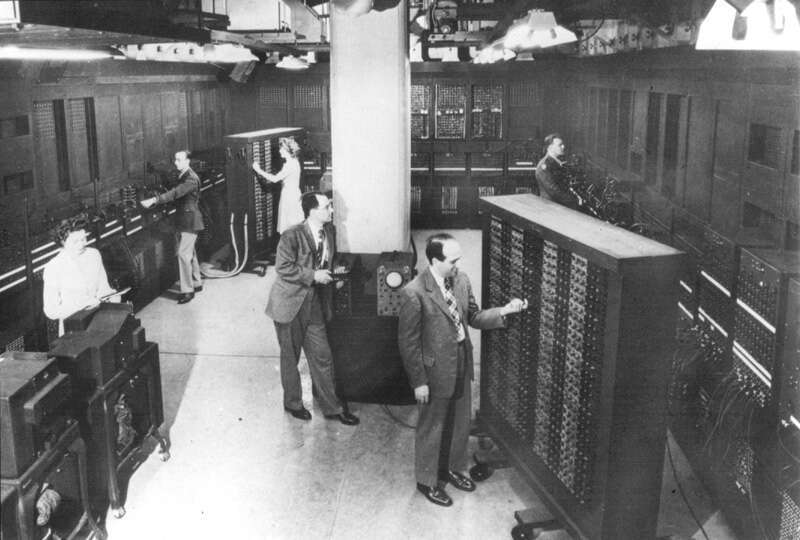
\includegraphics[width=0.6\textwidth]{pics/eniac.jpg}
\end{figure}
\newpage
\subsection{The Computer Keyboard}
One of the key parts of a computer that is still highly used today is the keyboard. Typewriters inspired keyboards. The typewriter has been around since the late 1800s and is an antique that is still used today. The QWERTY keyboard layout, which came from the Sholes and Glidden typewriter, also came from this time. QWERTY’s design has the keys to be spread out to avoid jamming those old typewriters. The QWERTY layout has stood the test of time in the English speaking world. The Binac computer (1948) used an electromechanically controlled typewriter to input data directly onto magnetic tape and print results. Binac’s typewriter was the first integration of a keyboard like system for a computer and began the computer keyboard’s origins. Since this origins, the keyboard is used in most electronic devices that require typing. 
\cite{ref3}

\begin{figure}[h!]
    \caption{The Binac Computer}
    \label{image:BINAC}
    \centering
    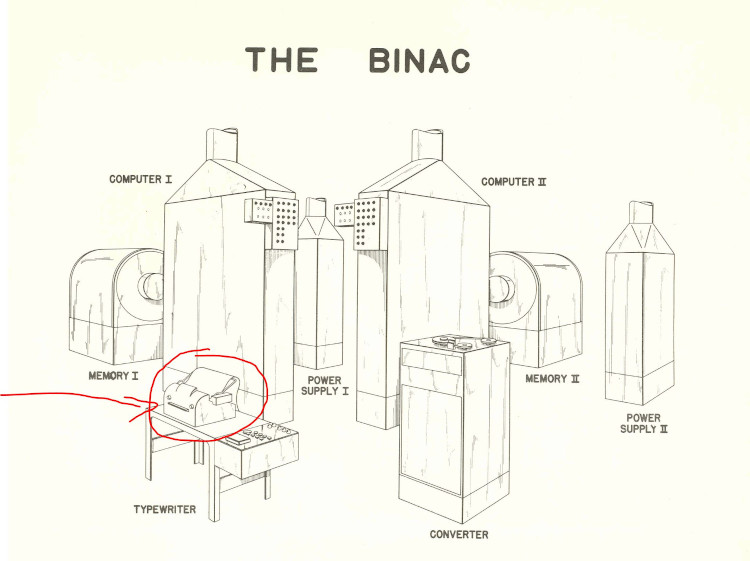
\includegraphics[width=0.45\textwidth]{pics/binac.jpg}
\end{figure}

\subsection{The Computer Screen}
What is a UI without a screen? A screen is so essential now and is probably the most important part of a computer. The ZUSE 3 (Z3) Computer (1941) was the first working programmable and fully automatic digital computer.  The Z3 was constructed with hundreds of relays, second-hand sheet metal, and mechanical pins. The Z3 had an output display that showed results on a light stripe, including the location of decimal commas. At the same time, computers from this time provided hard-copy printouts. Computers like the Z3 were dominated by a digital display that consisted of rows of blinking lights that flashed when the computer processed particular instructions or accessing memory locations. 
\cite{ref4} \cite{ref5}

\begin{figure}[!h]
    \caption{The ZUSE 3 Computer}
    \label{image:ZUSE3}
    \centering
    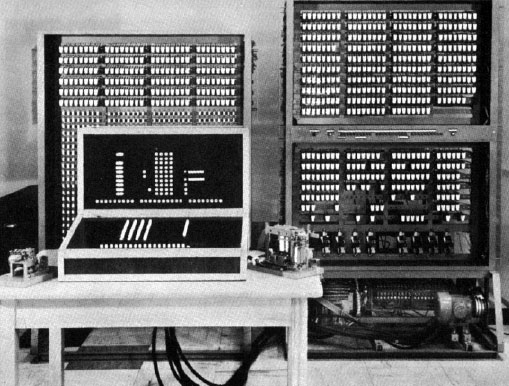
\includegraphics[width=0.5\textwidth]{pics/z3.jpg}
\end{figure}

In the 1980s, computer screens became revolutionary with CGA (Colour Graphics Adapter) and EGA (Enhanced Graphics Adapter) introduced by IBM. These brought color and higher resolution to computer screens. Followed by these displays, the Macintosh Monitors came, and they used bitmapped graphics. The Mac II’s (1978) video standard was quite similar to the VGA (Video Graphics Array). 

Also, in the 1980s, LDC (Liquid Crystal Display) screens that originated from the 1960s became widely used on calculators and watches with monochrome displays—from the 1980s and on through the 1990s, LCD drastically improved. At this time, LCD created a market boom for laptops. LDC is continued to be supported and used today in electronic devices such as PCs, laptops, TVs, smartphones, smartwatches, cameras, Etc.
\cite{ref5}

\begin{figure}[!h]
    \caption{Modern Screens}
    \label{image:MODERNSCREENS}
    \centering
    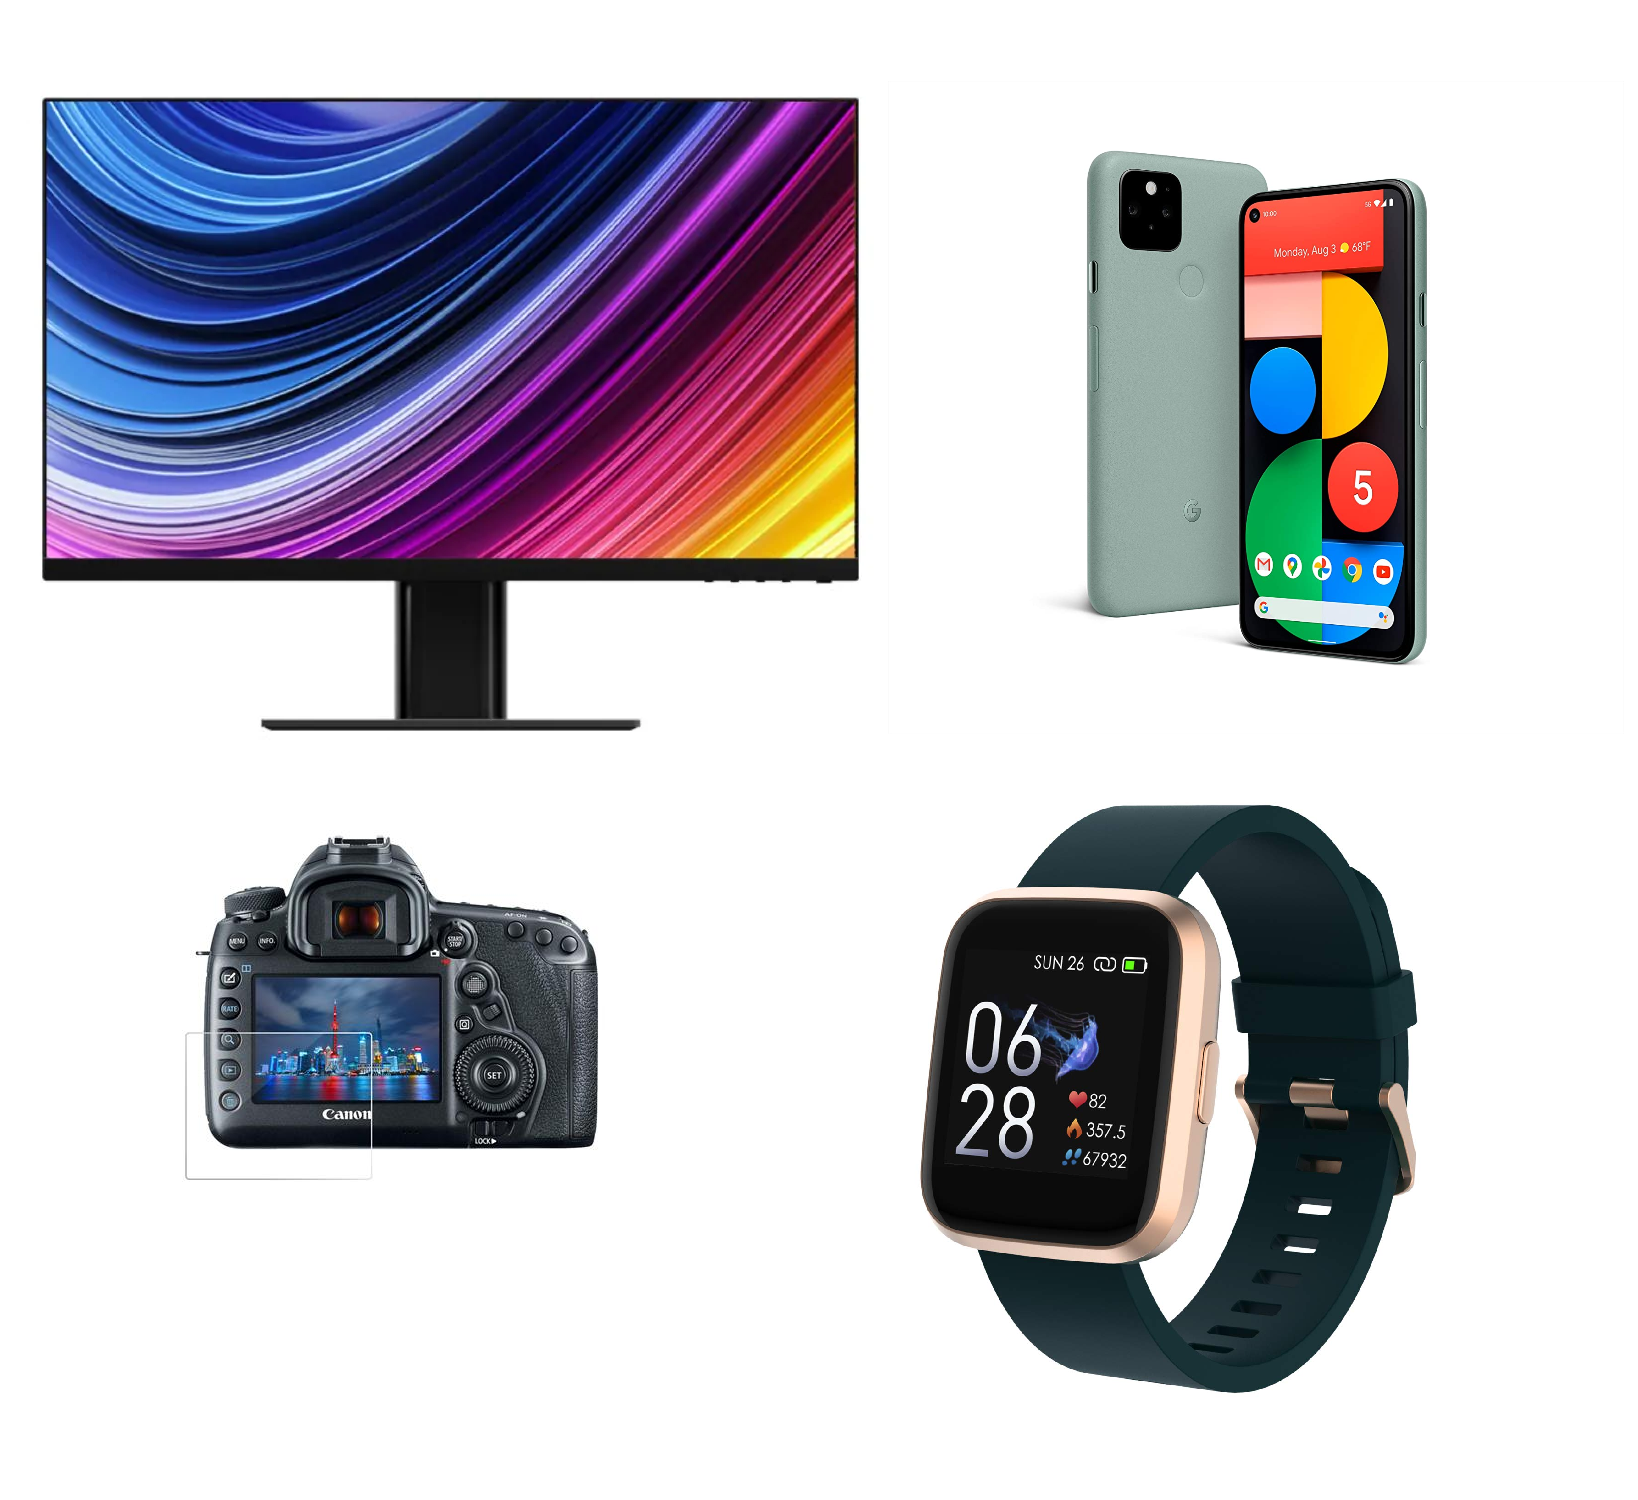
\includegraphics[width=0.3\textwidth]{pics/modern_screens.png}
\end{figure}

\subsection{The Computer Mouse}
The Mouse is another essential part of a computer. Before the use of the mouse, data was entered by typing commands with the keyboard, as discussed earlier. The standard mice that are used today are made out of plastic. The first computer mouse was a wooden box with two metal wheels that contact the surface and only one key. Douglas Engelbart invented this mouse in 1964. This mouse was pretty limited in what it could do. It was only eight years later that Bill English created the Ball Mouse. The ball replaced the two metal wheels that Engelbart’s mouse, which made it possible for this mouse to move in every direction. The Alto (1973) had a special input interface made by SRI. Alto’s mouse had three buttons and enabled the first bitmapped and overlapping windows display. As a result, Alto’s became very popular with its users. D. Venolia of Apple developed the first scroll-wheel in the late 1980s. It was not until the 1990s that mice started to resemble present-day mice. In 1999 Microsoft created a mouse known as the Intellimouse with an Optic LED design. This mouse paved the way for a new generation of optical mice.
\cite{ref6} \cite{ref7}

\begin{figure}[!ht]
    \caption{Computer Mice Throughout the Years}
    \label{image:mice}
    \centering
    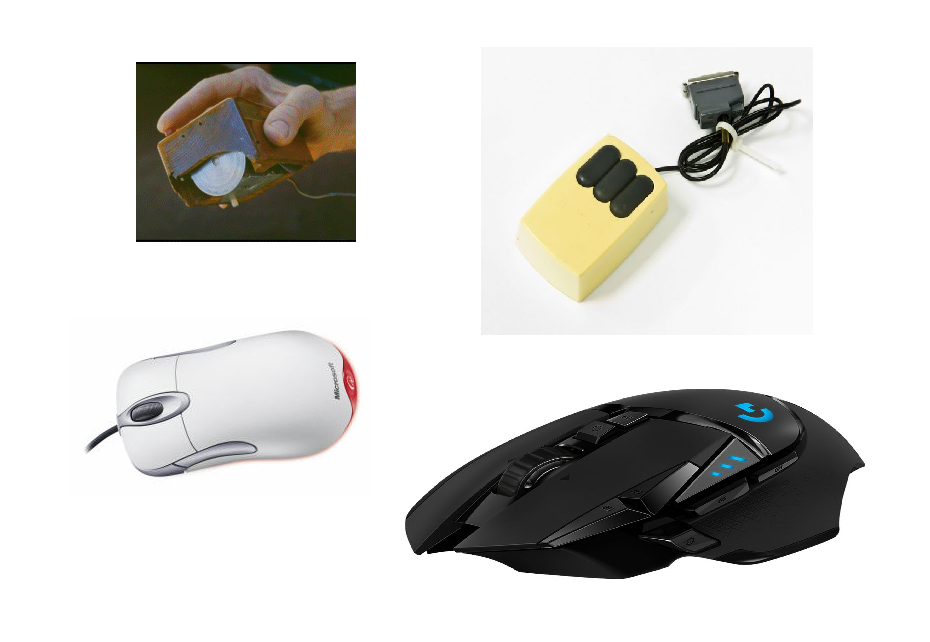
\includegraphics[width=0.45\textwidth]{pics/mice.png}
\end{figure}

\newpage
\subsection{The Touch Screen}
Throughout the years, touch screen technology has been vastly popular. There are touchscreens everywhere. They can be seen on PCs, laptops, smartphones, smartwatches, cameras, and almost every other electronic device. In the 1960s, the touchscreen emerged. In 1965, E.A.  Johnson invented the first touchscreen powered by fingertips. In many smartphones today, this touchscreen feature is used and is now known as the capacitive touch. The capacitive touchscreen display utilizes an insulator covered with a clear conductor, such as glass (Indium Tin Oxide).
Usually, a human finger or a touch pen is the ‘conductive’ component. By 1971, numerous various touchscreen computers were introduced. Plato IV, the first touchscreen device used in a classroom, was one of these computers. This computer allowed students to touch the screen to select answers to questions. Infrared technology was used in the PLATO IV rather than capacitive or resistive.
\cite{ref8}

\begin{figure}[!ht]
    \caption{The PLATO IV touchscreen terminal}
    \label{image:PLATOIV}
    \centering
    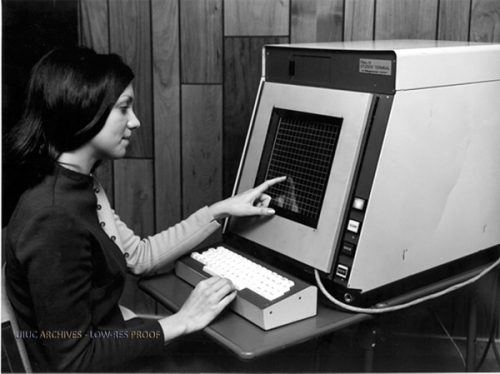
\includegraphics[width=0.5\textwidth]{pics/plato_iv.jpg}
\end{figure}

Touchscreens started to become highly commercialized at the beginning of the 1980s. HP developed a machine named the HP-150 in 1983. The HP-150 used MS-DOS and featured an infrared (IR) emitter surrounded by a 9-inch Sony CRT, and detectors sensed where the user’s finger came down from the screen. The HP-150 was not embraced immediately because it had problems with usability. For example, poking at the screen would block other IR rays that might tell the machine where the user's finger was pointing.

IBM and BellSouth partnered up in 1993 to launch the Simon Personal Communicator (SPC). One of the first cellphones that had a touchscreen was the SPC. The phone included paging capabilities, an application for e-mail and calendar, an appointment schedule, an address book, a calculator, and a sketchpad based on a pen. The touchscreen was resistive, requiring a stylus to navigate and input data from menus.
\cite{ref8}

\begin{figure}[!ht]
    \caption{IBM's Simon Personal Communicator}
    \label{image:SPC}
    \centering
    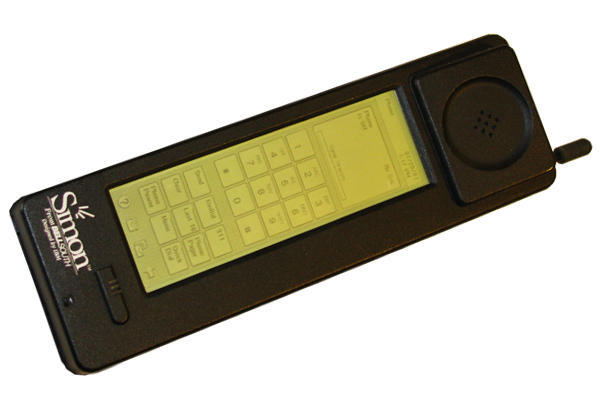
\includegraphics[width=0.5\textwidth]{pics/IBM_Simon.jpeg}
\end{figure}

Touchscreen technologies exploded in the 2000s. At this time, some developments helped introduce multi-touch and gesture based technologies to the people. The 2000s were also the period that touchscreens became the preferred collaboration platform for design. The arrival of PortfolioWall mainly targeted 3D animators and designers. PortfolioWall was a large-format touchscreen designed to be a dynamic variant of the boards used to monitor projects by design studios. The PortfolioWall was quick and easy-to-use with a gesture based interface. Users were able to examine and manage pictures, videos, and 3D files.
\cite{ref8}

\begin{figure}[!ht]
    \caption{PortfolioWall}
    \label{image:PFW}
    \centering
    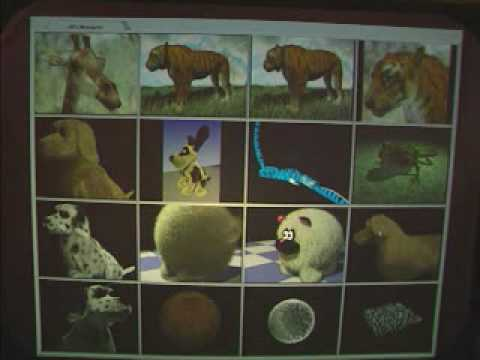
\includegraphics[width=0.4\textwidth]{pics/pf_wall.jpg}
\end{figure}

In 2007 Microsoft introduced the Surface at the All Things D conference. Although many of its design concepts were not new, it very effectively illustrated the real-world use case for touchscreens embedded into something the size of a coffee table. Microsoft designed the Surface to be used by their commercial customers to give users a sample of the hardware. Firms such as AT\&T used the Surface to display the latest handsets to buyers visiting their brick and mortar retail locations.

These technologies cannot be understated, as each had a monumental impact on the electronic devices we use today. Everything from PCs, laptops, smartphones, smartwatches, and cameras can connect to the numerous innovations and discoveries in touchscreen technology history.
\cite{ref8}

\subsection{Voice Recognition Control}
Compared to the other technologies mentioned earlier, Voice Control Recognition (VRC) seems relatively new. Like the touchscreen, VRC has been around since the middle of the 20th century. It is only in the past decade that it has taken its toll. Voice control is becoming more and more prominent. It has even inspired some films. The 2013 film ‘Her’ directed by Spike Jonze, starring Joaquin Phoenix and Scarlet Johansson, has an AI operating system that can learn and adapt. Pheonix plays Theodore, who is a writer, and Johansson plays the AI OS. They have deep, meaningful conversations in the film that show how advanced this AI OS is and possibly show where this technology’s future is going. 
\cite{ref9}

\begin{figure}[H]
    \caption{Her (2013) - Theodore and Samantha}
    \label{image:HER}
    \centering
    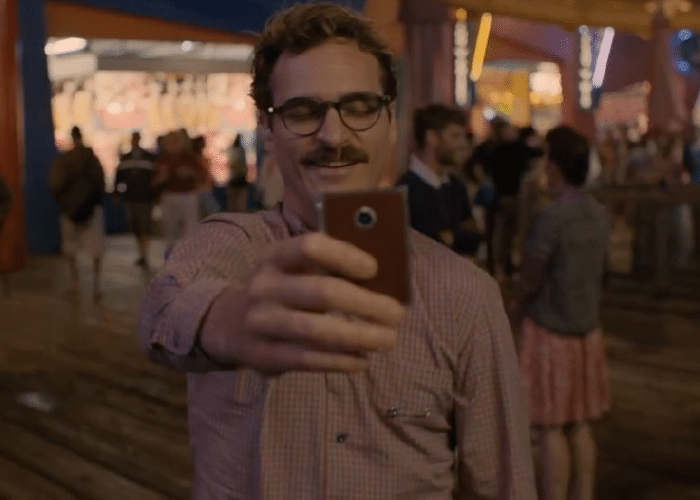
\includegraphics[width=0.45\textwidth]{pics/Her.png}
\end{figure}

One of the first uses of VRC was In 1939 with the Voder. The Voder was developed to synthesize human speech by imitating the human vocal cords’ effects, controlled by selecting one of the machine’s two basic sounds with the pedal bar. The Audrey, which recognized a limited choice of spoken digits, was developed by Bell Labs in 1952. Audrey could distinguish between zero and nine. “Audrey could recognize the sound of a spoken digit – zero to nine – with more than 90\% accuracy.”. IBM created the Shoebox in the early 1960s. The Shoebox had the ability to understand up to 16 spoken words in English. The Shoebox was operated by speaking into a microphone, which then converted sounds into electrical impulses.

In 1971, IBM created the Automatic Call Identification System, allowing engineers to talk to and accept spoken answers from a device, paving the first voice recognition steps. In 1976, The Harpy, developed by Carnegie Mellon of DARPA, registered 1,011 words. Similar to the other technologies mentioned earlier, VRC had a big boom in the 1980s. Hidden Markov Model was a new technique that allowed voice recognition machines to more accurately identify speech. Soon after this, IBM produced the Tangora, which was able to identify 20,000 spoken words. 

With the rise of AI and personal assistants in the 2000s, machine learning is enhancing VRC. In 2008, Google developed the Voice Search App for the iPhone, while Siri was introduced in 2011, giving their customers their own digital personal assistant. These enhancements marked a drastic change for mobile companies, as VRC enabled users to control their devices more efficiently than ever before. A few years after these devices, Microsoft introduced Cortana and Amazon created the Echo. With technologies like machine learning, VRC is only getting more advanced and heavily affects the future of electronic devices.
\cite{ref10}

\begin{figure}[!ht]
    \caption{Voice Recognition Control}
    \label{image:VRC}
    \centering
    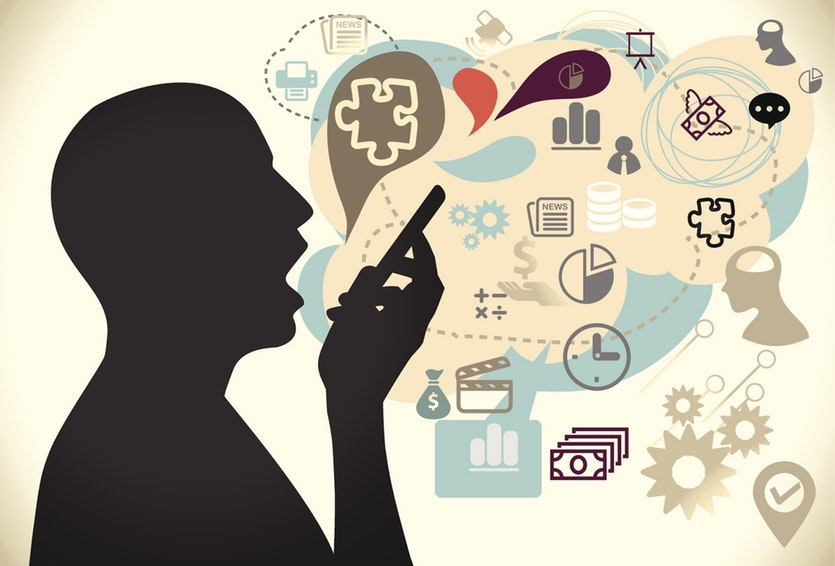
\includegraphics[width=0.4\textwidth]{pics/vrc.jpg}
\end{figure}

\subsection{Virtual and Augmented Spaces}
Virtual and Augmented Reality has given people the power to enter different worlds by just putting on a VR or AR headset. VR is an entirely virtual world. AR being a profound technology is the betterment of the old and the new as it enables a whole new world by blending the physical world with the virtual. These technologies were born when Charles Wheatstone invented the stereoscope in 1838. Wheatstone’s invention allowed the viewer to look at two similar images to create a 3D effect.
\cite{ref11}

\begin{figure}[H]
    \caption{Charles Wheatstone’s stereoscope}
    \label{image:stereoscope}
    \centering
    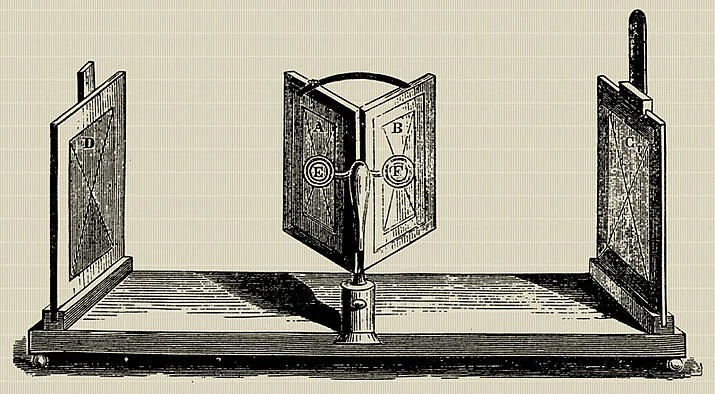
\includegraphics[width=0.5\textwidth]{pics/stereoscope.jpg}
\end{figure}

In 1960, Morton Heilig created the first-ever head-mounted display by inventing the Sensorama. This invention used stereoscopic technology and 3D imaging and widescreen vision, and stereo sound. In 1961, Philco Corporation created the Headsight built on Morton Heilig’s Sensorama. The Headsight was built mainly for the military. The Headsight allowed the remote viewing of possibly hazardous situations without putting people in danger.
\cite{ref11}

\begin{figure}[H]
    \caption{The Headsight}
    \label{image:Headsight}
    \centering
    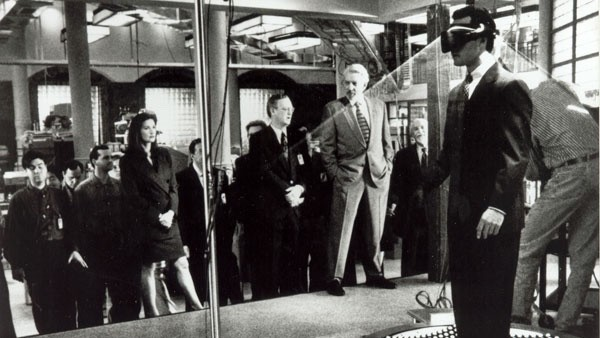
\includegraphics[width=0.6\textwidth]{pics/Headsight.jpg}
\end{figure}

VR was used in the early 1990s to build arcade games and revealed the technology to the public. The introduction of the first commercial VR system called the Sega VR followed these VR arcade games. The Sega VR was a home console that featured stereo sound and head tracking. Due to an excessive amount of headaches and motion sickness complaints, while using it, the Sega VR did not catch on.

There are both VR and AR applications in almost every field that can help organizations develop new training methods, communication opportunities, interactive models, and more. Films and Games use AR and VR as they have never have done before. AR and VR create a far more immersive experience for their users, and as a result, they are growing to be very popular. 
\cite{ref11}

\subsection{Gesture Recognition}
The invention of touchscreens described earlier has brought Gesture Recognition (GR) to a whole new level. GR’s origins were also discussed earlier, so modern uses of the technologies will be discussed here. GR has been quite prominent in video games. The Nintendo Wii brought GR to gaming’s center stage. The pairing of the Wii remote and the Wii sensor bar indicated the console could register a person’s movements and map them in a 3D computer-generated space. With the PlayStation, Sony soon followed the Wii by bringing out the Move and Eye technology similar to Nintendo’s GR work. Microsoft’s Xbox 360 Kinect camera took GR one step further. Its camera allows the Xbox 360 to recognize and track 20 individual joints of the human body. 
\cite{ref12}

In education, GR has shown tremendous promise. Hui-Mei Hsu (2011) provided a complete review of the usage of Kinect in education and concluded that it could produce the desired benefits, increase engagement and involvement in the classroom, and improve how teachers can control multimedia resources during classes.

The Myo is a drastic improvement from other motion control devices that use sensors to track gestures. Myo uses electromyography to interpret electrical signals from the wearer’s forearm muscles, map them with movements made by the wearer's hand, and monitor other instruments with certain gestures. For the Myo, it is not likely to be impaired by factors such as inadequate lighting conditions, space, and obstructions, unlike most GR devices using cameras. 
\cite{ref13}

GR technology will continue to evolve through enhancements and become even more widely used as they become more accessible with these enhancements.

\begin{figure}[!ht]
    \caption{The Myo}
    \label{image:MYO}
    \centering
    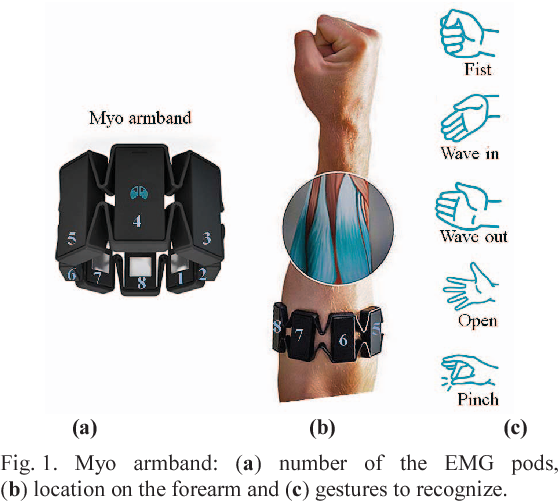
\includegraphics[width=0.4\textwidth]{pics/myo.png}
\end{figure}

\newpage
\section{Gestures as a Communication Tool}
% How are gestures used in everyday life for communication with others? They
% are a universal tool, albeit without a unilateral meaning and interpretation.
% How are gestures defined and become accepted to represent various aspects of
% communication?

Gestures have become a part of everyday communication. People do it naturally without thinking. Gestures go hand and hand with talking. They allow people to express themselves further.
Gestures do have their advantages and disadvantages. One major disadvantage is language barriers. For example, a gesture could mean something in one language and then mean something entirely different in another. One gesture that can bring some confusion is the ‘Okay’ gesture. In most English-speaking countries, this means okay, whereas, in Japan, it symbolizes money. In the Arab world, this sign’s shaking represents the evil eye and is used as a curse or a threat, sometimes combined with verbal condemnation. The ‘Come here’ gesture, usually done by the index finger, is used quite a lot in English speaking countries. In the Philippines, it is only used for dogs as it is believed to be derogatory to use on people, and people could get arrested for using it. Just from these two gestures, it is shown that how different they can be when they look the same and can cause miscommunication.
\cite{ref14}

\section{Challenges for the Design of Applications}
% Incorporating gestures is an important part of the design phase. Using the
% wrong gestures will leave users confused and frustrated as they learn a new
% system. The functionality of the system has to be appropriately mapped to
% the gesture set available in such a way to reduce the learning curve and the
% resistance gradient of the user

In Applications, Gestures are the new clicks. These gestures obtain a close personal connection with the content and improve the direct manipulation of on-screen objects. Designers have to be careful with applications as gestures can vary in what they mean and, unfortunately, limit the number of gestures in an application. However, this issue is not necessarily bad as the gesture will be more remember-able for users as there are only a few implemented. As users are accustomed to everyday gestures and do not like being challenged to learn many ways to do the same thing, this is a complex design environment. A pleasant aspect of the experience could be custom gestures in games and other immersive applications. It is easier to use familiar gestures in other apps because additional effort is not needed to discover or remember them.
\cite{ref15}

\section{Challenges for Implementation}
% Deciding that a particular gesture should carry out a particular function is one
% thing. Tracking that gesture and deciding when it has been made is a
% different challenge. Looking at some systems and the gestures they use, what
% are the challenges in implementation that had to be overcome for those systems?
% How were those challenges met (if they were met)?

Many smartphones rely on taps and swipes. They come very naturally to most people. These taps can be more than one to perform various functions. “In general, having a single action available on swipe-right that starts or progresses the most important task is recommended, and - optionally - a single action is made available on left swipe.”
\cite{ref16}
For implementing these navigation tools, developers had to take many things into account, such as what does one tap, two taps, or a swipe do? The navigation bar that is usually on Android phones has three inter-grated buttons. The functions of these buttons can be customized. Their standard functionalities are to go back, to view the app menu, and to see already opened apps. IOS devices do the same thing but with a single button and swipes. The Android navigation bar can be hard to use initially, but there is more control from these three buttons than the IOS setup. These are two similar devices intended to do the same thing, and they both do them differently.

\section{Conclusion}
% Conclusions are what you have learned from your research. This is your reflection on the current state of the art and the possible future directions of gesture-based user interfaces.

Throughout this paper, User Experience Evolution, Gestures as a Communication Tool, Challenges for the Design of Gesture Applications, and the Challenges for Implementation of Gestures were all discussed. By doing this research paper, I learned that the user interface has a long and exciting history. It was enjoyable to learn where the devices that are around us today originated. Gesture Based technology is a fascinating area of the modern world, and doing this paper, has inspired me to always keep an eye out for these devices and be up to date and their current status.
It is exciting to think about where these technologies might be in the future and how advanced they will be. Above everything else, I wholeheartedly believe machine learning will help these technologies become better with time and hard work from humans and machines. 
\newline
\newline
“The times are coming when a machine will stand there and remain at rest. A human being will approach it, knowing that he must make one movement of the hand in this way, another in a definite relation to it, and a third again; and through the pulsations in the air which thus arise out of a certain sign, the motor, being attuned to this particular sign, will be set in motion.” - Rudolf Steiner \cite{ref17}

%%% END OF CONTENT %%%%

\newpage
\begin{thebibliography}{00}
    
\bibitem{ref1} History of Computers
\newline
URL: \url{https://homepage.cs.uri.edu/faculty/wolfe/book/Readings/Reading03.htm}

\bibitem{ref2} Suzanne Deffree - EDN - Construction begins on ENIAC
\newline
URL: \url{https://www.edn.com/construction-begins-on-eniac-may-31-1943/}

\bibitem{ref3} Mary Bellis - The History of the Computer Keyboard
\newline
URL: \url{https://www.thoughtco.com/history-of-the-computer-keyboard-1991402}

\bibitem{ref4} History Computer Konrad Zuse
\newline
URL: \url{https://history-computer.com/konrad-zuse/}

\bibitem{ref5} Benji Edwards - PC World - A Brief History of Computer Displays
\newline
URL: \url{https://www.pcworld.idg.com.au/slideshow/366677/brief-history-computer-displays/}

\bibitem{ref6} Jessica Z - Sutori - History of the Computer Mouse
\newline
URL: \url{https://www.sutori.com/story/history-of-computer-mouse--2yUFPn6vNQBstaaz2x4FTdsy}

\bibitem{ref7} Bill Buxton - Some Milestones in Computer Input Devices
\newline
URL: \url{https://www.billbuxton.com/inputTimeline.html}

\bibitem{ref8} Florence Ion - From touch displays to the Surface
\newline
URL: \url{https://tinyurl.com/ycpwsg8m}

\bibitem{ref9} Spike Jonze - Her (2013)
\newline
URL: \url{https://g.co/kgs/vr9BSs}

\bibitem{ref10} Condeco - The History of Voice Recognition Technology
\newline
URL: \url{https://www.condecosoftware.com/blog/a-history-of-voice-recognition-technology/}

\bibitem{ref11}  Stephanie Baskerville - A Brief History of Virtual and Augmented Reality
\newline
URL: \url{https://www.proserveit.com/blog/history-of-virtual-and-augmented-reality}

\bibitem{ref12} Gesture Recognition Blog
\newline
URL: \url{https://blog.iinet.net.au/gesture-recognition/}

\bibitem{ref13} University of Birmingham - Gesture Control Technology
\newline
URL: \url{https://tinyurl.com/y68fdjw7}

\bibitem{ref14} Bright Side - 15 Hand Gestures That Have Different Meanings Overseas
\newline
URL: \url{https://tinyurl.com/yxl6kcw9}

\bibitem{ref15} Apple Developer - Gestures
\newline
URL: \url{https://tinyurl.com/y9zkjmpa}

\bibitem{ref16} Microsoft Docs - Implementation Tips for Gestures
\newline
URL: \url{https://tinyurl.com/y2p5trby}

\bibitem{ref17} Rudolf Steiner - The Insertion of Early Human Destiny into Extraterrestial Relationships
\newline
URL: \url{https://wn.rsarchive.org/Lectures/GA172/English/ZS3295/ZS3295_index.html} 

\end{thebibliography}

%%% CONTENT HERE END %%%%
\end{document}
\newpage
\setstretch{1}  %reduce bibliography line spacing
\printbibliography
\end{document}